\documentclass[11pt]{article}
\usepackage[margin=1in]{geometry}
\usepackage[T1]{fontenc}
\usepackage{amsmath}
\usepackage{xcolor}
\usepackage{listings}


\usepackage{tikz}
\usetikzlibrary{arrows.meta}

\lstset{
  basicstyle=\ttfamily\footnotesize,
  breaklines=true,
  frame=single,
  numbers=left,
  numberstyle=\tiny\color{gray},
  columns=fullflexible,
  keepspaces=true,
  showstringspaces=false,
  tabsize=4
}

\setlength{\parindent}{0pt}
\setlength{\parskip}{0.6em}

\lstdefinestyle{mystyle}{
    backgroundcolor=\color{backcolour},   
    commentstyle=\color{codegreen},
    keywordstyle=\color{magenta},
    numberstyle=\tiny\color{codegray},
    stringstyle=\color{codepurple},
    basicstyle=\ttfamily\footnotesize,
    breaklines=true,                 
    captionpos=b,                    
    keepspaces=true,                 
    numbers=left,                    
    showspaces=false,                
}
\lstset{style=mystyle}
\title{\textbf{COMP 321: Deliverable 2}\\ \Large  Initial complete solution}
\author{Raina Hu (261068856), Jessie Qiao (261176070) \& Jessica Xu (261163415)}

\date{}

\begin{document}
\maketitle

\section*{Deliverable 2.1}

\subsection*{Problem Statement}

\textbf{Awkward-Free Photo}\\\\
Every December, Bob hosts the office secret Santa party. Each guest draws a card from a bowl to find out which coworker they must give a gift to.\\
\\
This year Bob had far too much to drink while preparing for the party. He forgot to remove cards from the bowl, and guests tossed their cards back after drawing. As a result, some guests will receive several gifts, while others will receive none at all. At least nobody drew their own name.\\
\\
Bob wants to take a group photo with as many guests as possible. However, if guest $i$ gives a gift to guest $j$, it would be awkward for the two of them to stand in the same photo, since the surprise would be spoiled. (It does not matter who gives to whom: if either one gives to the other, they cannot both be in the photo. If they give to each other, it is still only one conflict.)\\
\\
Help Bob find the largest possible group of guests such that no guest in the group gives a gift to another guest in the group.

\subsubsection*{Input}

The first line contains an integer $n$ ($2 \le n \le 10^5$), the number of guests. The guests are numbered from $1$ to $n$.

The second line contains $n$ integers $a_1, a_2, \dots, a_n$ ($1 \le a_i \le n$ and $a_i \ne i$), where $a_i$ is the guest that guest $i$ gives a gift to.

\subsubsection*{Output}

Output a single integer: the maximum number of guests that can appear in the photo, that is, the size of the largest group of guests in which no guest gives a gift to another guest of the group.


\subsection*{Sample Input 1}
\begin{verbatim}
5
2 1 2 3 4
\end{verbatim}

\subsection*{Sample Output 1}
\begin{verbatim}
1
\end{verbatim}

\noindent Guest 1 gives to 2, guest 2 gives to 3, and guest 3 gives to 1. Every pair of guests is in conflict, so only one guest can be in the photo.

\subsubsection*{Sample Input 2}
\begin{verbatim}
6
2 3 1 1 1 2
\end{verbatim}

\subsubsection*{Sample Output 2}
\begin{verbatim}
4
\end{verbatim}

\noindent Guests 3, 4, 5 and 6 can be in the photo together: none of them gives a gift to another one of them. No group of 5 works.

\subsubsection*{Sample Input 3}
\begin{verbatim}
4
2 3 4 1
\end{verbatim}

\subsubsection*{Sample Output 3}
\begin{verbatim}
2
\end{verbatim}

\noindent\textbf{Time Limit:} 1.0 second

\noindent\textbf{Memory Limit:} 512 MB


\newpage

\section*{Solution Explanation}

We want the largest set of vertices with no edge between any two of them. This is the \textbf{Maximum Independent Set} (MIS) problem.

\subsection*{Modelling the input as a graph}
Treat every guest as a vertex and draw an edge from guest $i$ to guest $a_i$ (``$i$ gives a gift to $a_i$''). Every vertex has \emph{exactly one} outgoing edge. A graph with this property is called a \emph{functional graph}.

\begin{figure}[h]
    \centering
    % Source of figure.png (the figure in problem.tex).
% Build: pdflatex figure.tex && pdftoppm -r 300 -png -singlefile figure.pdf figure
\documentclass[tikz,border=6pt]{standalone}
\usepackage{tikz}
\usetikzlibrary{arrows.meta}
\begin{document}
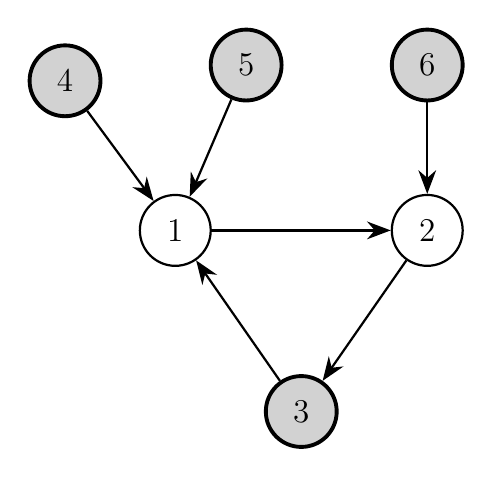
\begin{tikzpicture}[
    >={Stealth[length=3mm]},
    guest/.style={circle, draw, thick, minimum size=9mm, inner sep=0pt, font=\large},
    chosen/.style={guest, fill=gray!35, line width=1.4pt},
    gift/.style={->, thick}
]
  % the cycle
  \node[guest]  (1) at (0,0)     {1};
  \node[guest]  (2) at (3.2,0)   {2};
  \node[chosen] (3) at (1.6,-2.3) {3};
  % the trees hanging off the cycle
  \node[chosen] (4) at (-1.4,1.9) {4};
  \node[chosen] (5) at (0.9,2.1)  {5};
  \node[chosen] (6) at (3.2,2.1)  {6};

  \draw[gift] (1) -- (2);
  \draw[gift] (2) -- (3);
  \draw[gift] (3) -- (1);
  \draw[gift] (4) -- (1);
  \draw[gift] (5) -- (1);
  \draw[gift] (6) -- (2);
\end{tikzpicture}
\end{document}

    \caption{The gift graph of the second sample. An arrow from $i$ to $j$ means that guest $i$ gives a gift to guest $j$. The shaded
    guests $3, 4, 5, 6$ form a largest possible photo group.}
    \label{fig:sample2}
\end{figure}

\paragraph{Explanation of the samples.}
In the first sample, guests $1$ and $2$ give to each other, and guests $3$, $4$, $5$ form a chain $5 \to 4 \to 3 \to 2$. A largest group is $\{1, 3, 5\}$. In the second sample (see Figure~\ref{fig:sample2}), guests $1$, $2$ and $3$ give gifts in a circle, so at most one of them can be in the photo, and guests $4$, $5$ and $6$ can all join if guest $3$ is the chosen one. No group of five guests works.\\\\
Input: $n = 6$, $a = [2, 3, 1, 1, 1, 2]$. The edges are $1\text{--}2$, $2\text{--}3$, $3\text{--}1$, $4\text{--}1$, $5\text{--}1$, $6\text{--}2$.
\begin{itemize}
    \item Leaves $4, 5, 6$ are peeled first. Guests $4$ and $5$ push into $1$, guest $6$ pushes into $2$. Afterwards $\mathrm{in}[1] = 1$, $\mathrm{out}[1] = 2$, $\mathrm{in}[2] = 1$, $\mathrm{out}[2] = 1$, and $\mathrm{in}[3] = 1$, $\mathrm{out}[3] = 0$. No other vertex reaches in-degree $0$, so $\{1, 2, 3\}$ is the cycle.
    \item Case A (guest 1 taken): the best total is $2$.
    \item Case B (guest 1 not taken): the best total is $4$ (take $3, 4, 5, 6$).
\end{itemize}
The answer is $\max(2, 4) = 4$.




\paragraph{Why each tree has a single root on the cycle.}
Every guest has exactly one outgoing edge, so the path starting at any guest is unique. For a guest $v$ not on a cycle, this path enters a cycle at exactly one vertex $r$, the first cycle vertex it reaches. Hence every non-cycle guest belongs to the tree of exactly one cycle vertex, and no tree is attached to two cycle vertices (that would require a guest with two outgoing edges). For the same reason a connected component contains exactly one cycle: from a cycle vertex the only outgoing edge stays on the cycle, so a path can never leave one cycle to reach another.


\end{document}